\documentclass[longbibliography]{revtex4-2}

%\usepackage[margin=2cm]{geometry}
\usepackage{amsmath, amsfonts, amssymb}
\usepackage{hyperref}
\usepackage{graphicx}
\usepackage{subfigure}

\newcommand{\im}[0]{\mathfrak{i}}

\begin{document}

\title{Numerical analysis of quantum many-body scars and many-body localized
discrete time crystals}
\author{Anupam Mitra}
\date{2026-10-01}

\maketitle

\section{Introduction}\label{introduction}

Both many-body localized discrete time crystal (MBL-DTC), and quantum
many body scars (QMBS), involve revivals of an initial state during
time evolution. In the context of MBL-DTC, this is interpreted as period
doubling or symmetry breaking of time-translational symmetry as the
initial state is revived after two periods of the drive. In the context
of QMBS, this is interpreted as the result of constrained dynamics due
to the nearest neighbor Rydberg blockade condition. In both cases, there
is a non-negligible \(\gg \mathcal{O}(2^{-n})\), probability of
returning to the initial state.

In MBL-DTC, the revivals are attributed to eigenstate order while in
QMBS, they are attributed to an approximate block diagonal structure of
the Hamiltonian. Perhaps, the approximate block diagonal structure leads
to revival probabilities being close to but not equal to \(1\).

In QMBS, there is a special band of energy eigenstates in the so-called
scarred subspace, which has properties that are distinct from the rest
of the energy eigenstates. These special band eigenstates have energy,
not just at the edges, but throughout the spectrum. These eigenstates
have surprisingly low entanglement entropies, as would \emph{not} be
expected from the properties of a chaotic Hamiltonian.

In MBL-DTC, the dynamics are determined by the Floquet operator of one
period of the drive. The eigenvalues of the Floquet operator are
unimodular complex numbers, and in the period-doubling MBL-DTC phase
they occur in pairs differing by a phase of $\pi$. This pairing is the
eigenstate-order signature of the phase~\cite{khemani2016phase,
else2016floquet}: it is exact in the ideal-pulse soluble limit, and
emergent though rigid for generic
disorder~\cite{yao2017discrete}, rather than a symmetry identity of the
driven Hamiltonian. Unlike QMBS, there is no special band and the
eigenstate order exists throughout the spectrum.

This manuscript describes the models and the numerical methods, implemented
in the \texttt{mbl\_eigen} package accompanying this
manuscript,\footnote{The \texttt{mbl\_eigen} package accompanying this
manuscript implements the model builders, eigenvalue-analysis workflows,
eigensolver backends, level-spacing statistics, and the Qiskit circuit and
simulation layer described in Sec.~\ref{sec:numerical-methods}. It is
distributed together with the source repository of this manuscript.} used to
study the eigenvalue structure and eigenstate ordering associated with these
two settings, together with the results obtained so far and the analyses that
remain to be completed.

\section{Review}\label{sec:review}

The QMBS phenomenology originates in the observation of long-lived
revivals of the N\'eel ordered initial state in the 51-atom Rydberg
quantum simulator of Ref.~\cite{bernien2017probing}, and the controlled
driven dynamics of Ref.~\cite{bluvstein2021controlling} subsequently
established tunable access to this regime. The PXP Hamiltonian that
describes the blockade-constrained dynamics was then shown to exhibit a
weak breaking of ergodicity: a tower of special eigenstates, not
concentrated at the spectral edges but spread through the spectrum,
carries anomalously low entanglement entropies and distinct spectral
statistics~\cite{turner2018weak, turner2018quantum}. The scarred states
are nearly equally spaced in energy, and have been reinterpreted as
finite-energy-density condensates of weakly interacting
$\pi$-magnons~\cite{iadecola2019magnon}. Exact scarred eigenstates of
the PXP model were constructed in Ref.~\cite{lin2019exact}, the scarred
dynamics were shown to be governed by an emergent $SU(2)$ symmetry with
fine-tuned deformations producing perfect scars~\cite{choi2019emergent},
related constructions cover spin-$1$ XY magnets with subextensive
entanglement and spatiotemporal long-range order~\cite{schecter2019weak}
and Rydberg models in the antiblockade regime with emergent kinetic
constraints and finite-entanglement revivals~\cite{iadecola2020scar},
and scar states were identified in the deconfined regime of lattice
gauge theories, where extensive local constraints play the role of the
blockade condition~\cite{aramthottil2022scar}. The weak-ergodicity-breaking
picture of Ref.~\cite{serbyn2021quantum} and the quasiparticle perspective
of Ref.~\cite{chandran2023quantum} unify these
developments, treating scars as stable quasiparticle species throughout
the energy spectrum and placing them alongside symmetry-based
constructions, projector embeddings, and Hilbert-space fragmentation.

These eigenstates are significant as violations of expectations encoded
in the eigenstate thermalization hypothesis, under which the eigenstates
of a chaotic Hamiltonian behave as random variables, so that an initial
state built from them approaches thermal
equilibrium~\cite{srednicki1994chaos}. A quantitative benchmark is given
by the Page value: the subsystem entropy of a typical pure state of a
bipartite system is close to that of the maximally mixed reduced
state~\cite{page1993average}. The entanglement entropy of eigenstates
and the mean adjacent level-spacing ratio, the two diagnostics computed
in the workflows of Secs.~\ref{subsec:workflows}
and~\ref{subsec:level-spacing}, are the standard tools for locating
deviations from these expectations. The level-spacing ratio is
insensitive to the local density of states and therefore applies to
many-body spectra without unfolding~\cite{atas2013distribution}; the
crossover it detects, from Wigner-Dyson statistics characteristic of
chaotic spectra to Poisson statistics of integrable or localized ones,
has been used to diagnose many-body localization since
Ref.~\cite{oganesyan2007localization}.

The MBL-DTC descends from the Floquet phases with spatiotemporal
long-range order identified in Refs.~\cite{khemani2016phase,
else2016floquet}: in a periodically driven, strongly disordered spin
system, the Floquet eigenstates occur in cat doublets separated by a
quasienergy difference of $\pi$, and this eigenstate order underlies
the period-doubled response of local
observables~\cite{khemani2016phase}. The pairing is stable to all weak
local deformations of the drive, including ones that explicitly break
the defining symmetries of the soluble pulse models, which occupy
submanifolds of a larger absolutely stable
phase~\cite{vonkeyserlingk2016absolute}; this rigidity, together with
the criticality and candidate realizations of the phase, was analyzed
in Ref.~\cite{yao2017discrete}. The stabilizing mechanism is
many-body localization, whose phenomenology, including quasi-local
integrals of motion and the spreading of entanglement after quenches,
is reviewed in Ref.~\cite{abanin2019colloquium}. Experimentally,
discrete time-crystalline order was observed in a disordered dipolar
many-body system~\cite{choi2017observation}, in a trapped-ion spin
chain~\cite{zhang2017observationdiscrete}, in an ordered dipolar
system~\cite{rovny2018observation}, in a programmable spin-based
quantum simulator~\cite{randall2021many}, and on a superconducting
quantum processor~\cite{mi2022time}; a disorder-free prethermal
variant, stabilized by high-frequency driving rather than by
localization, was observed in a trapped-ion
simulator~\cite{kyprianidis2021observation}.

Interpreting propagator eigenvalues requires distinguishing two pairing
mechanisms, which I analyze in
Secs.~\ref{many-body-localized-discrete-time-crystal}
and~\ref{quantum-many-body-scars}. A chiral, or particle-hole, symmetry
of the Hamiltonian forces the spectrum to be symmetric under
$E \leftrightarrow -E$, so that propagator eigenvalues occur in
complex-conjugate pairs $\eta \leftrightarrow \eta^{*}$; at zero
detuning the PXP model realizes this mechanism through the
anticommuting particle-hole operator $\prod_{l} Z_{l}$
~\cite{turner2018weak}, and for Floquet unitaries chiral symmetry
likewise produces exact scarred multiplets~\cite{mizuta2020exact}. The
period-doubled MBL-DTC instead pairs quasienergies as
$\varepsilon \leftrightarrow \varepsilon + \pi$, so that propagator
eigenvalues occur in phase-$\pi$ pairs $\eta \leftrightarrow -\eta$;
this cat-doublet structure is an emergent eigenstate-order signature
rather than a symmetry identity of the driven
Hamiltonian~\cite{khemani2016phase, else2016floquet, yao2017discrete}.
The two pairings coincide only at special points, such as the DTC point
of the dipolar experiment of Ref.~\cite{choi2017observation}, where the
paired quasienergies cluster near $\pi/2$; away from such points the
distinction is sharp, and conflating the two would misattribute a
symmetry consequence to eigenstate order, or conversely.

The numerical methodology of this work draws on established traditions.
The level-spacing statistics of Sec.~\ref{subsec:level-spacing} and the
half-chain entanglement entropies compared against the maximally mixed
reference value in Sec.~\ref{subsec:workflows} follow the diagnostic
program outlined above~\cite{oganesyan2007localization,
atas2013distribution, page1993average}. The circuit layer of
Sec.~\ref{subsec:qiskit} continues a line of work in which scar and
time-crystal dynamics are implemented on gate-based quantum computers:
time-crystalline eigenstate order was probed on a superconducting
quantum processor~\cite{mi2022time}, and Trotterized simulations of
scar dynamics in Rydberg-blockade (PXP) chains have been demonstrated
on quantum hardware with pulse-level control and error
mitigation~\cite{chen2022error}.

Relative to this literature, the contribution of the present manuscript
is deliberately methodological. I do not propose new models and I do
not claim new eigenstate-order physics; rather, the
\texttt{mbl\_eigen} package implements, in one reusable code base, the
model builders of
Secs.~\ref{many-body-localized-discrete-time-crystal}
and~\ref{quantum-many-body-scars}, eigensolver backends spanning CPU
and accelerator devices, level-spacing statistics for both energy and
eigenphase spectra, entanglement diagnostics, and a Qiskit circuit and
simulation layer for the same propagators. The Floquet operator of the
MBL-DTC is constructed gate-natively, without Trotterization, while
the random-field MBL dynamics is synthesized as a first- or
second-order Trotter circuit, and the output conventions of
Sec.~\ref{subsec:reproducibility}, including seeded disorder sampling
and regression tests, make the figures of this manuscript traceable to
the code that produced them. The remainder of the manuscript documents
these methods in detail and the results obtained with them so far.

\section{Many-body localized discrete time crystal}\label{many-body-localized-discrete-time-crystal}

Many-body localized discrete time crystal (MBL-DTC) is a dynamical
phase of matter that can be seen in the driven dynamics of spin
models~\cite{ippoliti2021many, mi2022time, choi2017observation,
rovny2018observation, zhang2017observationdiscrete, randall2021many}.

A model where MBL-DTC is seen is the Floquet dynamics of a
one-dimensional Ising model with Floquet operator
\begin{equation}\label{eq:mbldtc-notes}
    U_{\mathrm{drive}}(\theta_x) =
    \left[\prod_{\ell=0}^{N-2}
    \exp\left(-\im\, \varphi_{zz,\ell}\,
    \frac{1}{4} Z_{\ell} Z_{\ell+1}\right)\right]
    \left[\prod_{\ell=0}^{N-1}
    \exp\left(-\im\, \varphi_{z,\ell}\,
    \frac{1}{2} Z_{\ell}\right)\right]
    \left[\prod_{\ell=0}^{N-1}
    \exp\left(-\im\, \theta_{x}\,
    \frac{1}{2} X_{\ell}\right)\right],
\end{equation}
where $\varphi_{z}$'s and $\varphi_{zz}$'s have spatial disorder and
$\theta_{x}$ is the same for all spins and corresponds to a control
parameter~\cite{ippoliti2021many, mi2022time}. This model shows
MBL-DTC for $\theta_x > 0.84\,\pi$ and shows thermalization for
$\theta_x < 0.84\,\pi$. I look for eigenstate ordering in the eigenvalues
of $U_{\mathrm{drive}}(\theta_x)$.

Since the MBL-DTC here corresponds to period doubling, the eigenstate
order corresponds to the eigenvalues of $U_{\mathrm{drive}}(\theta_x)$
differing by a phase of $\pi$: in the MBL-DTC dynamical phase, every
eigenvalue $\eta$ is paired with a partner
$\eta \mathrm{e}^{\im\pi} = -\eta$ obtained by multiplying by the
phase factor $\mathrm{e}^{\im\pi}$. This cat-doublet pairing is the
emergent eigenstate-order signature of the period-doubled phase, exact
in the ideal-pulse soluble limit and emergent though rigid for generic
disorder, rather than a symmetry identity of the driven
Hamiltonian~\cite{khemani2016phase, else2016floquet, yao2017discrete}.

I look for eigenstate order in a few instances of
$U_{\mathrm{drive}}(\theta_x)$.

\begin{figure}
  \centering
  \subfigure[sample: 1ce27428-2d40-41f7-9a71-ba3cce0ebc5b]{\includegraphics[width=0.46\textwidth]{../Plots/mbldtc_N=06_thetax=0.64pi_1ce27428-2d40-41f7-9a71-ba3cce0ebc5b.pdf}}
  \subfigure[sample: 5eb497b1-f406-4464-a0dc-335e3dab0edf]{\includegraphics[width=0.46\textwidth]{../Plots/mbldtc_N=06_thetax=0.64pi_5eb497b1-f406-4464-a0dc-335e3dab0edf.pdf}}
    \caption{$N=6$, $\theta_x=0.64\pi$. Eigenvalues $\eta$ (filled) and
      their complex conjugates $\eta^*$ (open), reflections about the
      real axis, of the Floquet operator; the phase-$\pi$ partners
      $-\eta$ associated with period doubling are not shown.}
\end{figure}

\begin{figure}
  \centering
  \subfigure[sample: 12f145dc-d2ec-464a-954d-a4abaa9fc5b2]{\includegraphics[width=0.46\textwidth]{../Plots/mbldtc_N=06_thetax=0.96pi_12f145dc-d2ec-464a-954d-a4abaa9fc5b2.pdf}}
  \subfigure[sample: 1aa00503-e25a-4276-a068-5075178cb219]{\includegraphics[width=0.46\textwidth]{../Plots/mbldtc_N=06_thetax=0.96pi_1aa00503-e25a-4276-a068-5075178cb219.pdf}}
  \caption{$N=6$, $\theta_x=0.96\pi$. Eigenvalues $\eta$ (filled) and
      their complex conjugates $\eta^*$ (open), reflections about the
      real axis, of the Floquet operator; the phase-$\pi$ partners
      $-\eta$ associated with period doubling are not shown.}
\end{figure}

\begin{figure}
  \centering
  \subfigure[sample: 228965e5-8f86-4b93-869c-5f6c7c77d391]{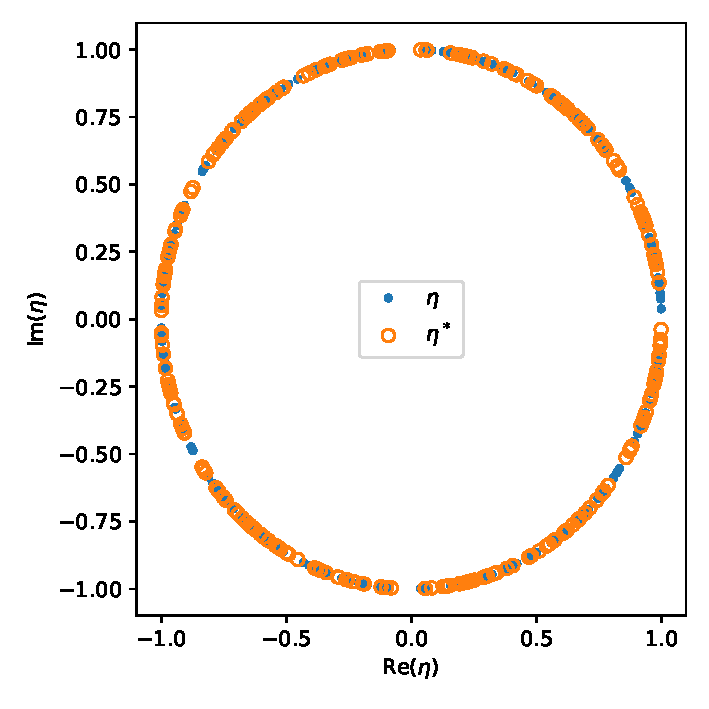
\includegraphics[width=0.46\textwidth]{../Plots/mbldtc_N=08_thetax=0.64pi_228965e5-8f86-4b93-869c-5f6c7c77d391.pdf}}
  \subfigure[sample: db04f039-0c77-41d8-b8cb-1d28fc64e514]{\includegraphics[width=0.46\textwidth]{../Plots/mbldtc_N=08_thetax=0.64pi_db04f039-0c77-41d8-b8cb-1d28fc64e514.pdf}}
  \caption{$N=8$, $\theta_x=0.64\pi$. Eigenvalues $\eta$ (filled) and
      their complex conjugates $\eta^*$ (open), reflections about the
      real axis, of the Floquet operator; the phase-$\pi$ partners
      $-\eta$ associated with period doubling are not shown.}
\end{figure}

\begin{figure}
  \centering
  \subfigure[sample: 078cd1bd-c55c-46bc-8a59-f087e72ceb17]{\includegraphics[width=0.46\textwidth]{../Plots/mbldtc_N=08_thetax=0.96pi_078cd1bd-c55c-46bc-8a59-f087e72ceb17.pdf}}
  \subfigure[sample: f20ee949-20bd-456a-9edf-eccbbc1d4c03]{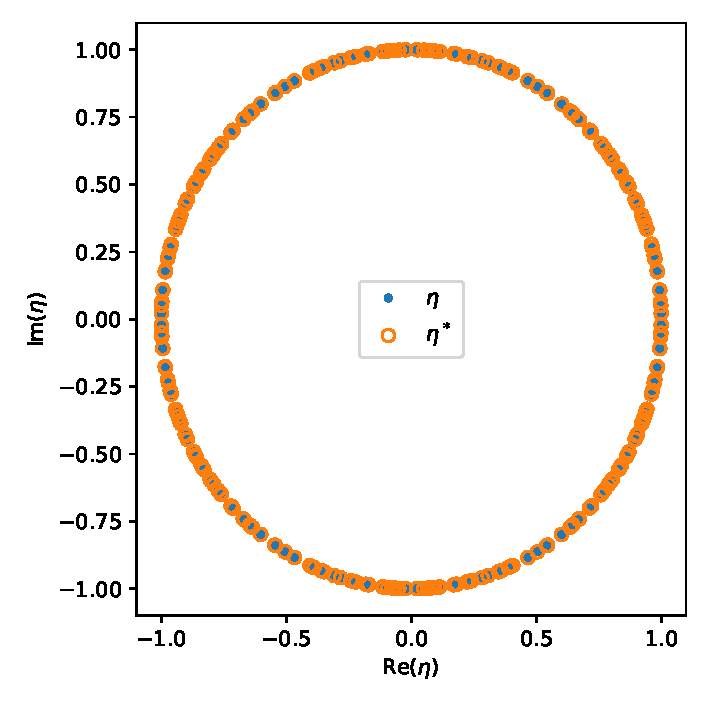
\includegraphics[width=0.46\textwidth]{../Plots/mbldtc_N=08_thetax=0.96pi_f20ee949-20bd-456a-9edf-eccbbc1d4c03.pdf}}
  \caption{$N=8$, $\theta_x=0.96\pi$. Eigenvalues $\eta$ (filled) and
      their complex conjugates $\eta^*$ (open), reflections about the
      real axis, of the Floquet operator; the phase-$\pi$ partners
      $-\eta$ associated with period doubling are not shown.}
\end{figure}

\begin{figure}
  \centering
  \subfigure[sample: 2a436997-d2e7-465d-8a66-522f4ad162af]{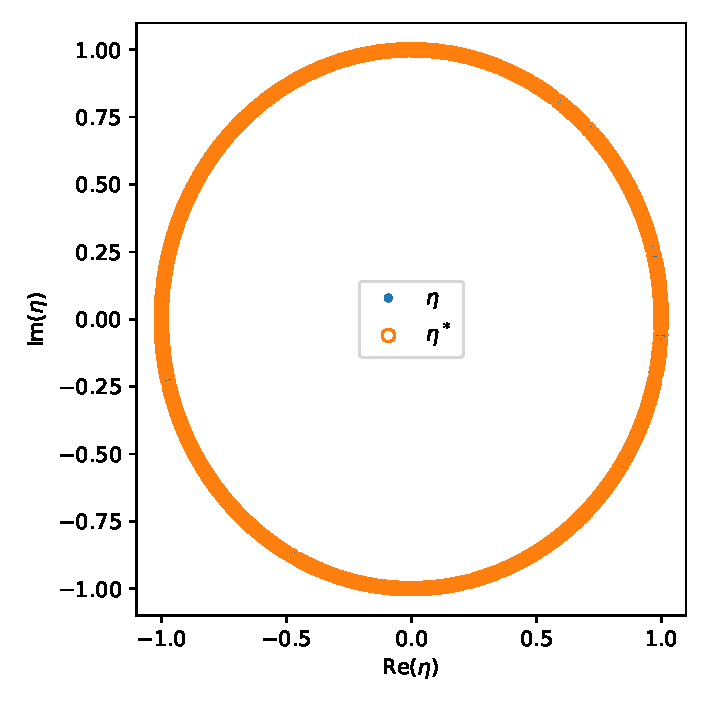
\includegraphics[width=0.46\textwidth]{../Plots/mbldtc_N=10_thetax=0.64pi_2a436997-d2e7-465d-8a66-522f4ad162af.pdf}}
  \subfigure[sample: fa3404ce-524f-4a9f-85c2-8315a6b19efb]{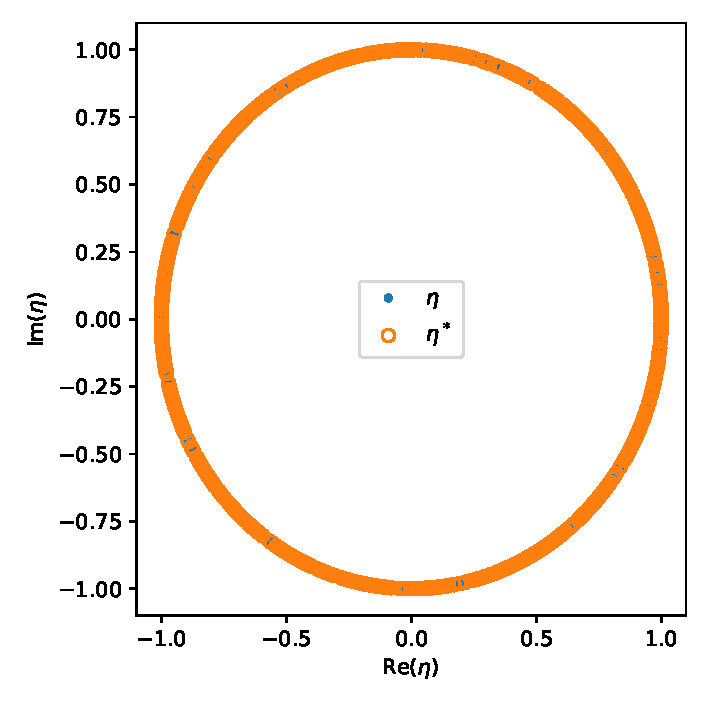
\includegraphics[width=0.46\textwidth]{../Plots/mbldtc_N=10_thetax=0.64pi_fa3404ce-524f-4a9f-85c2-8315a6b19efb.pdf}}
  \caption{$N=10$, $\theta_x=0.64\pi$. Eigenvalues $\eta$ (filled) and
      their complex conjugates $\eta^*$ (open), reflections about the
      real axis, of the Floquet operator; the phase-$\pi$ partners
      $-\eta$ associated with period doubling are not shown.}
\end{figure}


\begin{figure}
  \centering
  \subfigure[sample: 1366a22e-7e75-49e3-8dcf-96f76015aa14]{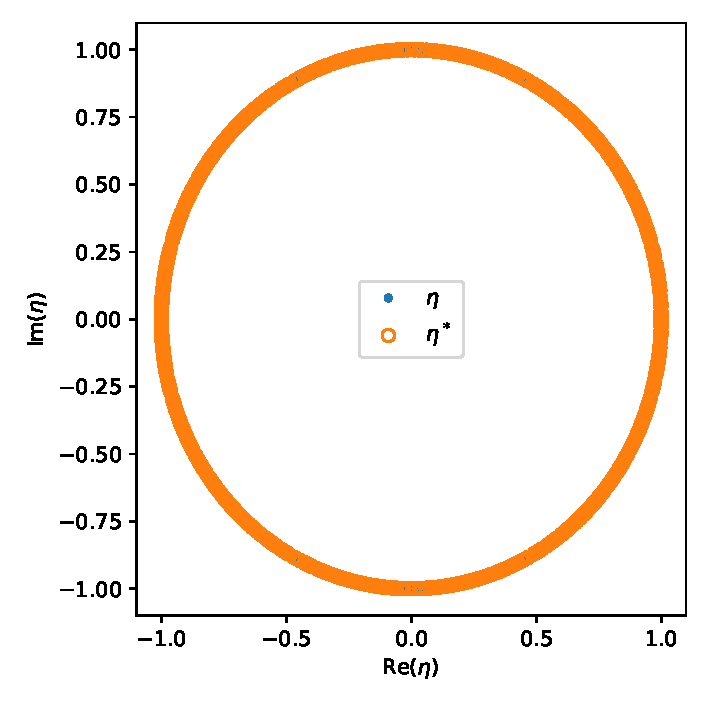
\includegraphics[width=0.46\textwidth]{../Plots/mbldtc_N=10_thetax=0.96pi_1366a22e-7e75-49e3-8dcf-96f76015aa14.pdf}}
  \subfigure[sample: d17e5ae9-1360-4254-b66e-7444d05b4a77]{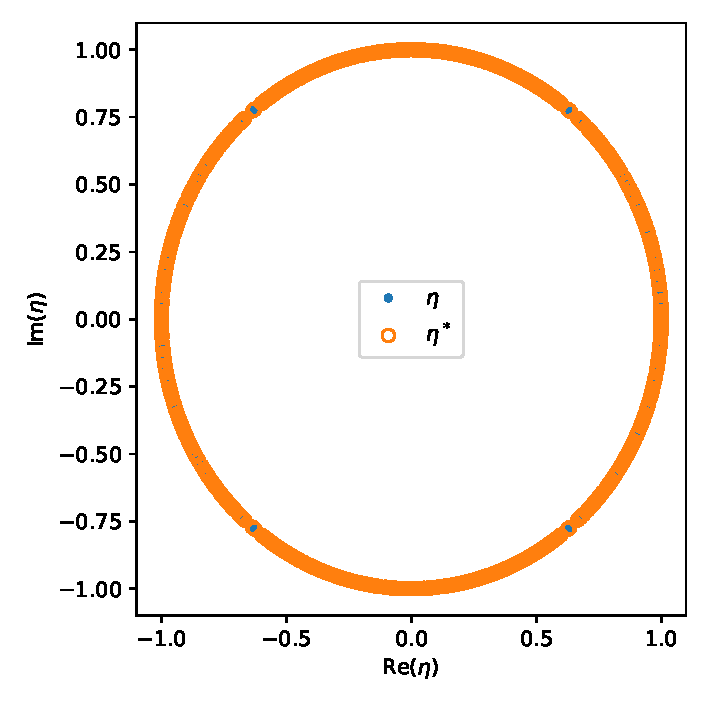
\includegraphics[width=0.46\textwidth]{../Plots/mbldtc_N=10_thetax=0.96pi_d17e5ae9-1360-4254-b66e-7444d05b4a77.pdf}}
  \caption{$N=10$, $\theta_x=0.96\pi$. Eigenvalues $\eta$ (filled) and
      their complex conjugates $\eta^*$ (open), reflections about the
      real axis, of the Floquet operator; the phase-$\pi$ partners
      $-\eta$ associated with period doubling are not shown.}
\end{figure}


\section{Quantum many-body scars}\label{quantum-many-body-scars}

Quantum many-body scars (QMBS) were discovered as an explanation for
periodic revivals of a N\'eel ordered initial state in a one-dimensional
array of neutral atoms with ground-to-Rydberg excitation
~\cite{bernien2017probing, bluvstein2021controlling}.

The Hamiltonian of this system in the basis of $| g \rangle$,
representing an atomic ground state and $| r \rangle$, representing an
atomic Rydberg state is effectively an Ising model with transverse and
longitudinal fields, which I call slanted field Ising
(SFI) model. For simplicity I consider the case of interactions only
between nearest neighbors when excited to atomic Rydberg states. In
the rotating frame at the angular frequency of the laser driving the
$| g \rangle \leftrightarrow | r \rangle$, transition and under the
rotating wave approximation, the Hamiltonian reads
\begin{equation}\label{eq:sfi-notes}
    H_{\mathrm{SFI}}
    =
    \frac{\Omega}{2} \sum_{l} X_{l} -
    \frac{\Delta}{2} \sum_{l} Z_{l} +
    V_{rr} \sum_{l} \left( \frac{1 + Z_{l}}{2} \right)
                    \left( \frac{1 + Z_{l+1}}{2} \right),
\end{equation}
where $\Omega$ is the Rabi frequency for, and $\Delta$ is the detuning
from, the $| g \rangle \leftrightarrow | r \rangle$ transition, and
$V_{rr}$ is the interaction between nearest-neighbor atoms when
excited to their Rydberg states.

A common regime of operation is the Rydberg blockade regime, which
occurs when $|V_{rr}| \gg \Omega$. In the nearest neighbor Rydberg
blockade and zero detuning $\Delta = 0$ regime, the system can be
described using a PXP model
~\cite{turner2018weak, turner2018quantum, maskara2021discrete},
whose Hamiltonian reads
\begin{equation}\label{eq:pxp-notes}
    H_{\mathrm{PXP}} = \Omega \sum_{l} P_{l-1} X_{l} P_{l+1},
\end{equation}
where $P_{l}$ represents the projector onto the ground state,
$| g \rangle \langle g |$ for the $l$-th atom, hence the name `PXP'
model. The PXP model is known to have QMBS. Therefore, I expect QMBS
to be seen in the SFI model, in an appropriately constrained part of
the Hilbert space.

To study this I consider quantum quenches, but instead of looking at
the time evolution of an initial state, I consider the time evolution
operators
\begin{equation}\label{eq:upxp}
    U_{\mathrm{PXP}}(t) = \exp\left(-\im t H_{\mathrm{PXP}}\right),
\end{equation}
and
\begin{equation}\label{eq:usfi}
    U_{\mathrm{SFI}}(t) = \exp\left(-\im t H_{\mathrm{SFI}}\right),
\end{equation}
for the PXP and SFI models respectively. I plot the eigenvalues, $\eta$
of these time evolution operators and their complex conjugates $\eta^*$.
The complex conjugate $\eta^* = \mathrm{e}^{+\im E t}$ is itself an
eigenvalue of the propagator $U(t) = \exp(-\im t H)$ only when the
spectrum of $H$ contains $-E$ (up to phase aliasing of
$\mathrm{e}^{-\im E t}$); it is guaranteed for every eigenvalue when the
spectrum of $H$ is symmetric under $E \leftrightarrow -E$, that is,
when the model has an energy-reflection symmetry,
that is, a unitary $S$ with $S H S^{\dagger} = -H$ (equivalently, a
chiral symmetry of the Floquet unitary); such a symmetry maps the
eigenvalue $\eta = \mathrm{e}^{-\im E t}$ of the state at energy $E$ to
the eigenvalue $\mathrm{e}^{+\im E t}$ of the partner state at energy
$-E$.

I find that across different durations, \(t\) and system sizes \(N\),
the eigenvalues of \(U_{\mathrm{PXP}}(t)\) are complex conjugate
pairs. This pairing is a symmetry consequence rather than an
eigenstate-order signature: at \(\Delta = 0\), the particle-hole
symmetry operator \(\Gamma = \prod_{l} Z_{l}\) anticommutes with every
PXP term \(P_{l-1} X_{l} P_{l+1}\), so
\(\{ \Gamma, H_{\mathrm{PXP}} \} = 0\) and the spectrum is symmetric
under \(E \leftrightarrow -E\)~\cite{turner2018weak}, which makes
\(\eta^*\) the eigenvalue of the partner state at energy \(-E\). The
longitudinal detuning term \(\Delta \sum_{l} Z_{l} / 2\) of the general
builder, Eq.~\eqref{eq:hpxp-code}, commutes with \(\Gamma\) and breaks
this anticommutation; the PXP figures shown here are \(\Delta = 0\)
outputs of an earlier version of the package, with legacy filenames
without an explicit detuning term
(Sec.~\ref{subsec:reproducibility}).

For \(U_{\mathrm{SFI}}(t)\), I find that a fraction of the eigenvalues
occur close to their complex conjugates. The SFI Hamiltonian of
Eq.~\eqref{eq:sfi-notes} has no energy-reflection symmetry for
\(V_{rr} \neq 0\), so the conjugate points are plotted as reflections
about the real axis, that is, as a guide to the eye, and no spectral
mechanism guarantees an overlap. In the parameter regime of the figures
(\(\Delta = 0\), \(V_{rr} = 100\,\Omega\)) the absence of such a
symmetry follows directly from the spectrum: the Rydberg-interaction
term \(V_{rr} \sum_{l} P_{r}^{(l)} P_{r}^{(l+1)}\) is positive
semidefinite, so \(E_{\min} \geq -\Omega N / 2\), while the all-Rydberg
product state has energy \(V_{rr} (N-1)\), so
\(E_{\max} \geq V_{rr} (N-1) > \Omega N / 2\); a spectrum invariant
under \(E \leftrightarrow -E\) would require
\(E_{\max} = -E_{\min} \leq \Omega N / 2\), a contradiction. Any
apparent overlap of \(\eta\) with \(\eta^*\) may reflect phase
aliasing, that is, eigenphases of large-magnitude \(E t\) wrapping
around the unit circle modulo \(2\pi\), rather than a spectral
symmetry.

In summary, two distinct pairing mechanisms act in this work. A chiral,
or particle-hole, symmetry, that is, a unitary \(\mathcal{P}\) with
\(\mathcal{P} H \mathcal{P}^{\dagger} = -H\) (equivalently,
\(\{\mathcal{P}, H\} = 0\) for \(\mathcal{P}^2 = \mathbb{1}\)), forces
the spectrum to be symmetric under \(E \leftrightarrow -E\), so that
propagator eigenvalues occur in
conjugate pairs \(\eta \leftrightarrow \eta^*\); this structure
underlies the exact scarred eigenstates of PXP-like and fine-tuned
models~\cite{turner2018weak, lin2019exact, choi2019emergent} and, for
Floquet systems, follows from a chiral symmetry of the Floquet
unitary~\cite{mizuta2020exact}. The period-doubled MBL-DTC phase
instead exhibits a cat-doublet structure that pairs quasienergies as
\(\varepsilon \leftrightarrow \varepsilon + \pi\), so that propagator
eigenvalues occur in phase-\(\pi\) pairs
\(\eta \leftrightarrow -\eta\); this pairing is the emergent
eigenstate-order signature of the phase rather than a symmetry
identity~\cite{khemani2016phase, else2016floquet}. For a generic
real-symmetric Hamiltonian, neither pairing is guaranteed.

\begin{figure}
  \centering
  \subfigure[SFI]{
    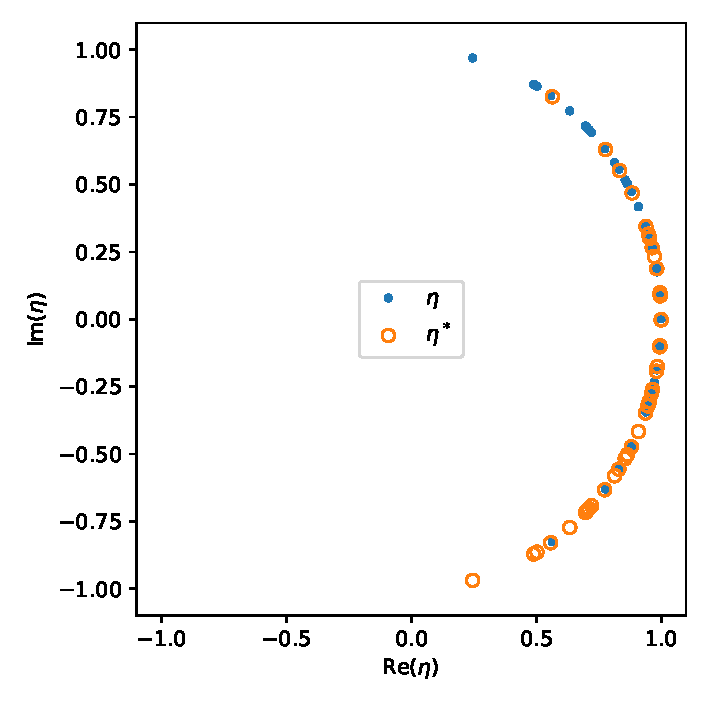
\includegraphics[width=0.44\textwidth]{../Plots/qmbs_sfim_N=06_tduration=0.5_Vrr=100_Omega=1.pdf}
  }
  \subfigure[PXP]{
    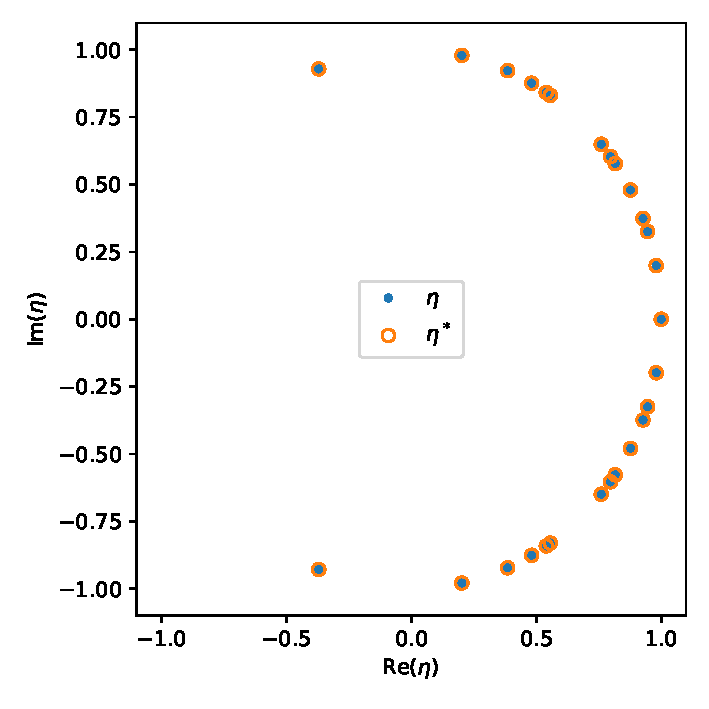
\includegraphics[width=0.44\textwidth]{../Plots/qmbs_pxp_N=06_tduration=0.5_Omega=1.pdf}
  }
  \caption{Eigenvalues $\eta$ (filled) and their complex conjugates
    $\eta^*$ (open) of the propagator, plotted in the complex plane for
    $N=6$, $\Omega t=0.5$. (a)~SFI with $V_{rr}=100\Omega$: the
    conjugates are reflections about the real axis, shown as a guide to
    the eye. (b)~PXP: the particle-hole symmetry
    $\Gamma = \prod_{l} Z_{l}$ of the PXP model at $\Delta = 0$ makes
    $\eta^*$ the eigenvalue of the partner state at energy $-E$.}
\end{figure}

\begin{figure}
  \centering
  \subfigure[SFI]{
    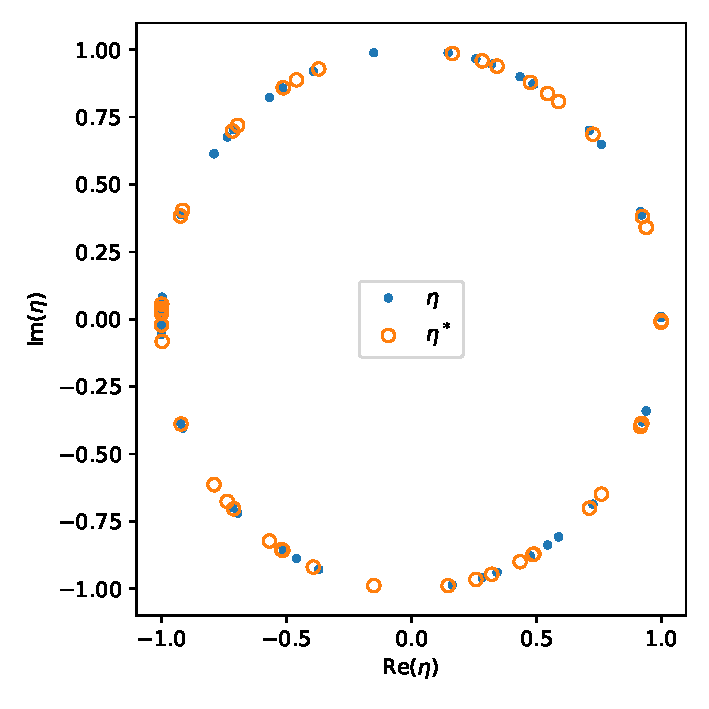
\includegraphics[width=0.44\textwidth]{../Plots/qmbs_sfim_N=06_tduration=2_Vrr=100_Omega=1.pdf}
  }
  \subfigure[PXP]{
    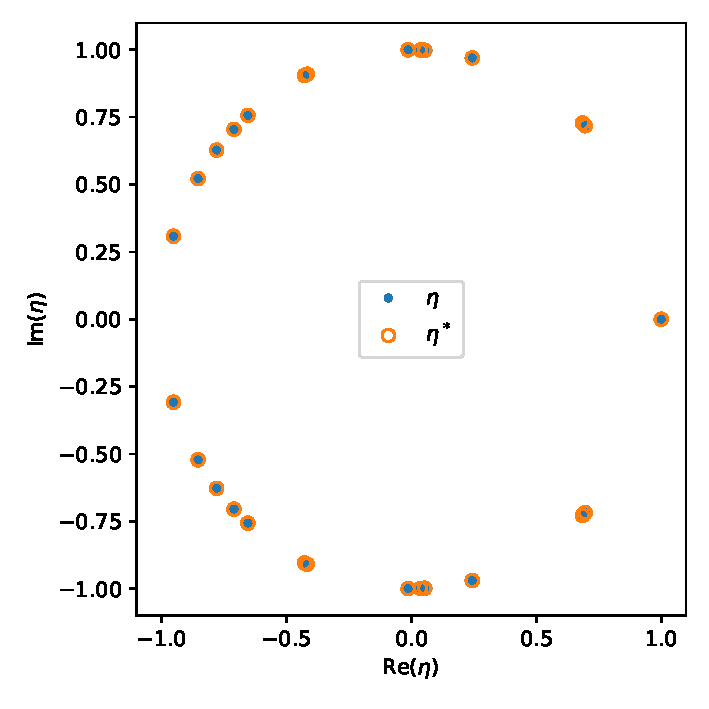
\includegraphics[width=0.44\textwidth]{../Plots/qmbs_pxp_N=06_tduration=2_Omega=1.pdf}
  }
  \caption{Eigenvalues $\eta$ (filled) and their complex conjugates
    $\eta^*$ (open) of the propagator, plotted in the complex plane for
    $N=6$, $\Omega t=2$. (a)~SFI with $V_{rr}=100\Omega$: the
    conjugates are reflections about the real axis, shown as a guide to
    the eye. (b)~PXP: the particle-hole symmetry
    $\Gamma = \prod_{l} Z_{l}$ of the PXP model at $\Delta = 0$ makes
    $\eta^*$ the eigenvalue of the partner state at energy $-E$.}
\end{figure}


\begin{figure}
  \centering
  \subfigure[SFI]{
    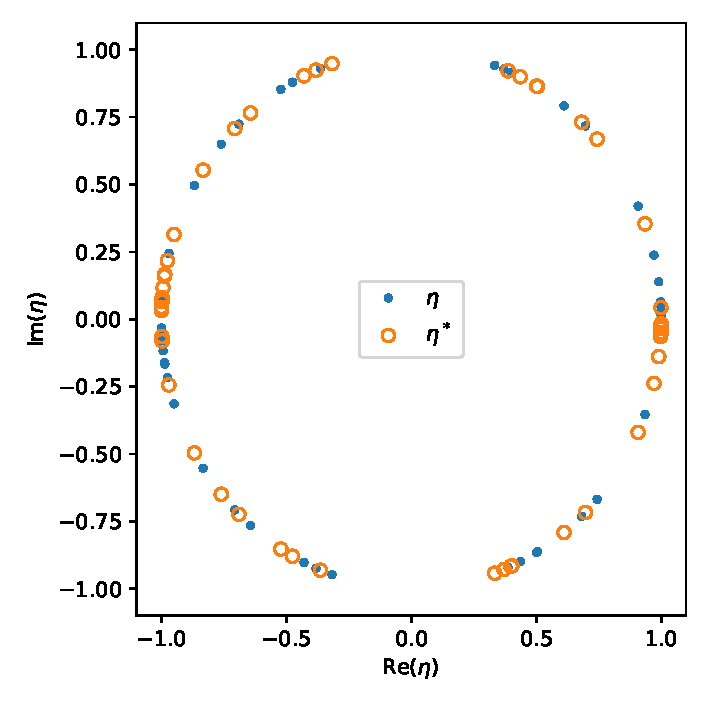
\includegraphics[width=0.44\textwidth]{../Plots/qmbs_sfim_N=06_tduration=6_Vrr=100_Omega=1.pdf}
  }
  \subfigure[PXP]{
    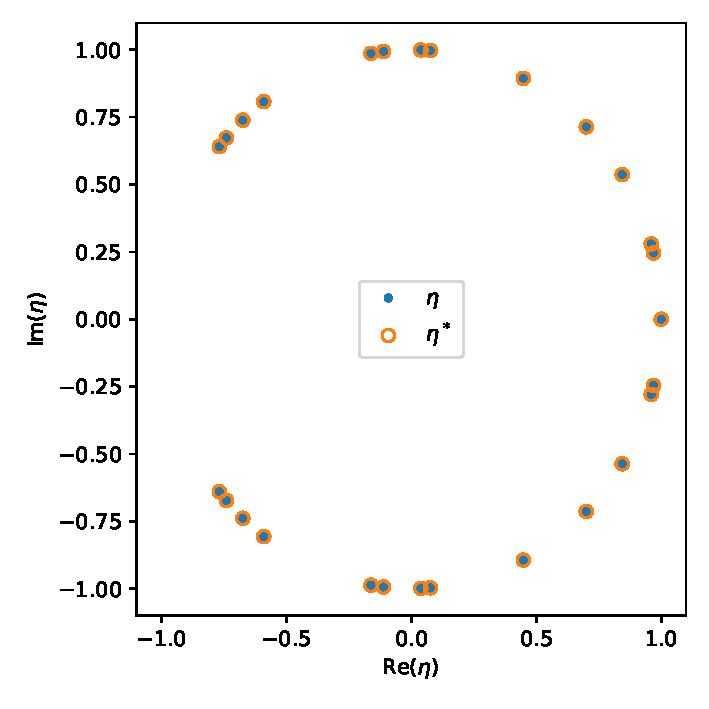
\includegraphics[width=0.44\textwidth]{../Plots/qmbs_pxp_N=06_tduration=6_Omega=1.pdf}
  }
  \caption{Eigenvalues $\eta$ (filled) and their complex conjugates
    $\eta^*$ (open) of the propagator, plotted in the complex plane for
    $N=6$, $\Omega t=6$. (a)~SFI with $V_{rr}=100\Omega$: the
    conjugates are reflections about the real axis, shown as a guide to
    the eye. (b)~PXP: the particle-hole symmetry
    $\Gamma = \prod_{l} Z_{l}$ of the PXP model at $\Delta = 0$ makes
    $\eta^*$ the eigenvalue of the partner state at energy $-E$.}
\end{figure}


\begin{figure}
  \centering
  \subfigure[SFI]{
    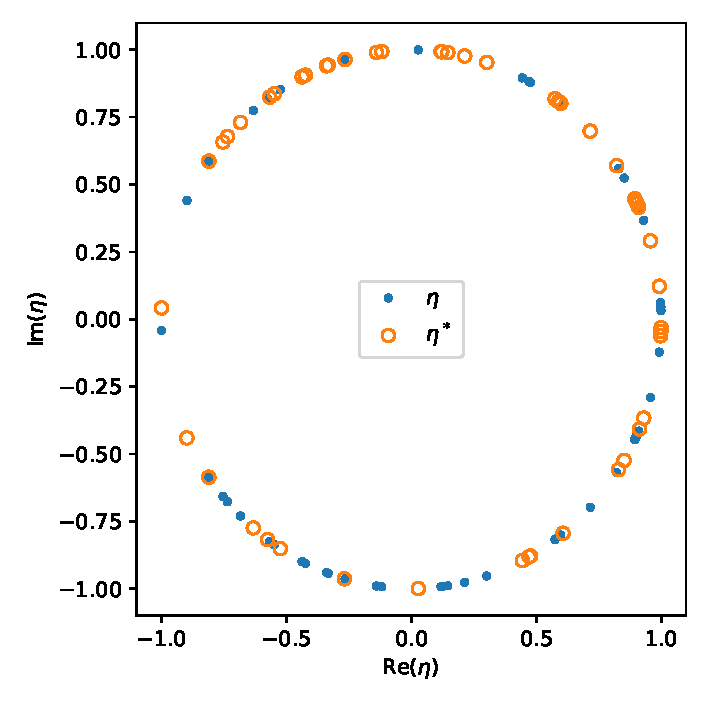
\includegraphics[width=0.44\textwidth]{../Plots/qmbs_sfim_N=06_tduration=11_Vrr=100_Omega=1.pdf}
  }
  \subfigure[PXP]{
    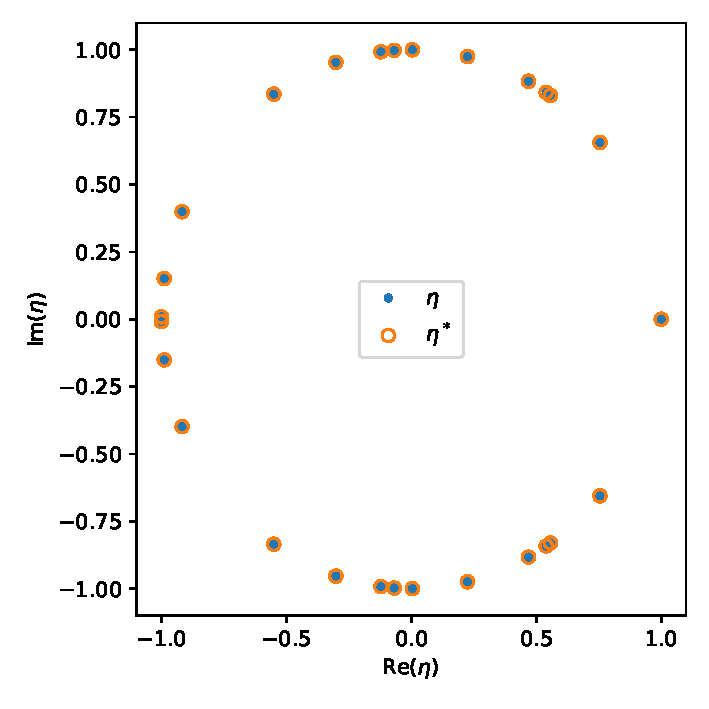
\includegraphics[width=0.44\textwidth]{../Plots/qmbs_pxp_N=06_tduration=11_Omega=1.pdf}
  }
  \caption{Eigenvalues $\eta$ (filled) and their complex conjugates
    $\eta^*$ (open) of the propagator, plotted in the complex plane for
    $N=6$, $\Omega t=11$. (a)~SFI with $V_{rr}=100\Omega$: the
    conjugates are reflections about the real axis, shown as a guide to
    the eye. (b)~PXP: the particle-hole symmetry
    $\Gamma = \prod_{l} Z_{l}$ of the PXP model at $\Delta = 0$ makes
    $\eta^*$ the eigenvalue of the partner state at energy $-E$.}
\end{figure}

%%%%%%%%%%%%%%%%

\begin{figure}
  \centering
  \subfigure[SFI]{
    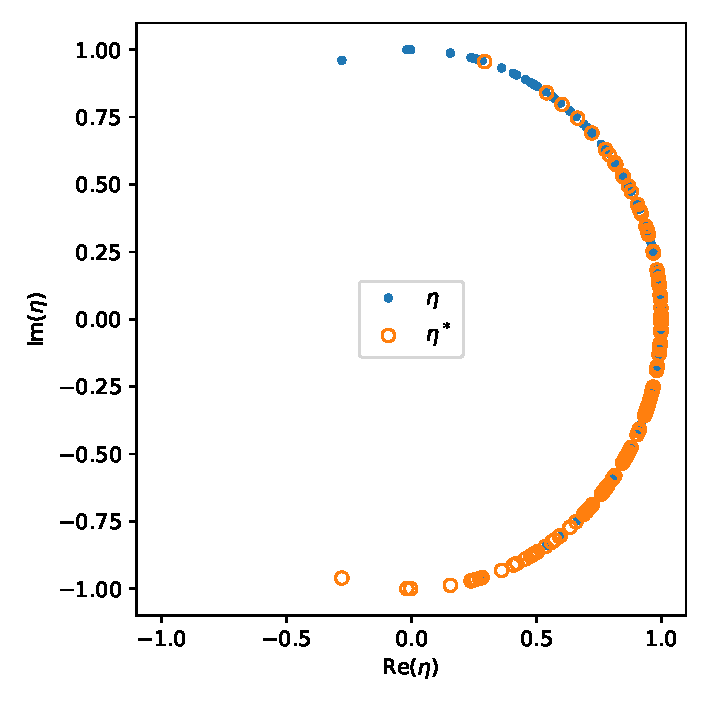
\includegraphics[width=0.44\textwidth]{../Plots/qmbs_sfim_N=08_tduration=0.5_Vrr=100_Omega=1.pdf}
  }
  \subfigure[PXP]{
    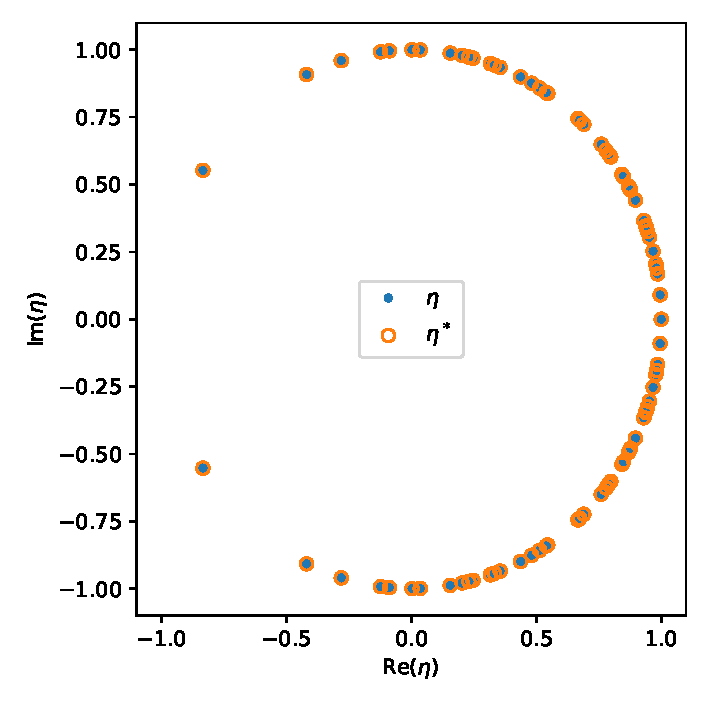
\includegraphics[width=0.44\textwidth]{../Plots/qmbs_pxp_N=08_tduration=0.5_Omega=1.pdf}
  }
  \caption{Eigenvalues $\eta$ (filled) and their complex conjugates
    $\eta^*$ (open) of the propagator, plotted in the complex plane for
    $N=8$, $\Omega t=0.5$. (a)~SFI with $V_{rr}=100\Omega$: the
    conjugates are reflections about the real axis, shown as a guide to
    the eye. (b)~PXP: the particle-hole symmetry
    $\Gamma = \prod_{l} Z_{l}$ of the PXP model at $\Delta = 0$ makes
    $\eta^*$ the eigenvalue of the partner state at energy $-E$.}
\end{figure}

\begin{figure}
  \centering
  \subfigure[SFI]{
    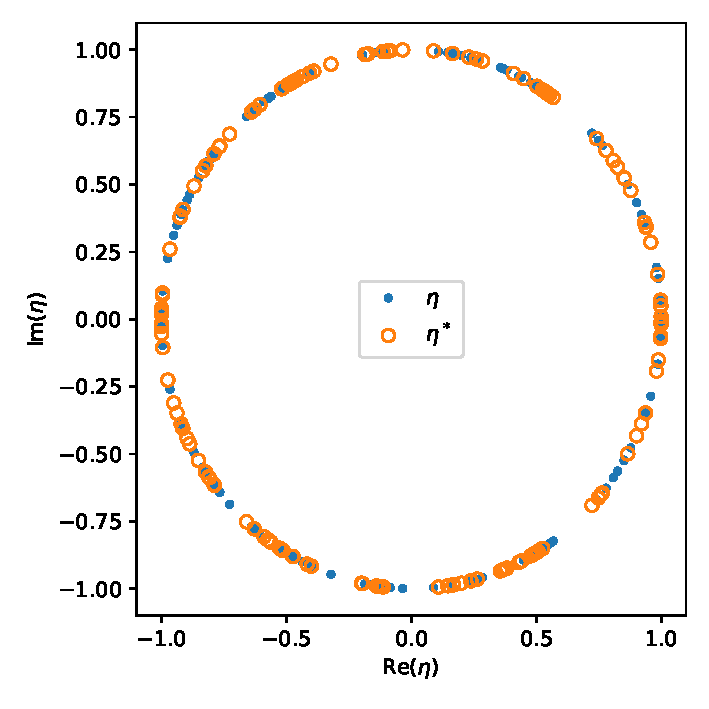
\includegraphics[width=0.44\textwidth]{../Plots/qmbs_sfim_N=08_tduration=2_Vrr=100_Omega=1.pdf}
  }
  \subfigure[PXP]{
    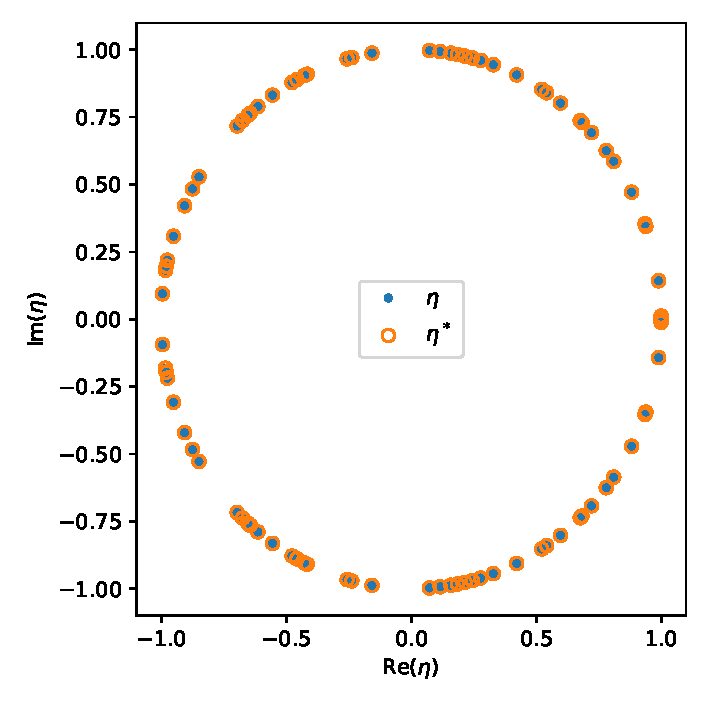
\includegraphics[width=0.44\textwidth]{../Plots/qmbs_pxp_N=08_tduration=2_Omega=1.pdf}
  }
  \caption{Eigenvalues $\eta$ (filled) and their complex conjugates
    $\eta^*$ (open) of the propagator, plotted in the complex plane for
    $N=8$, $\Omega t=2$. (a)~SFI with $V_{rr}=100\Omega$: the
    conjugates are reflections about the real axis, shown as a guide to
    the eye. (b)~PXP: the particle-hole symmetry
    $\Gamma = \prod_{l} Z_{l}$ of the PXP model at $\Delta = 0$ makes
    $\eta^*$ the eigenvalue of the partner state at energy $-E$.}
\end{figure}


\begin{figure}
  \centering
  \subfigure[SFI]{
    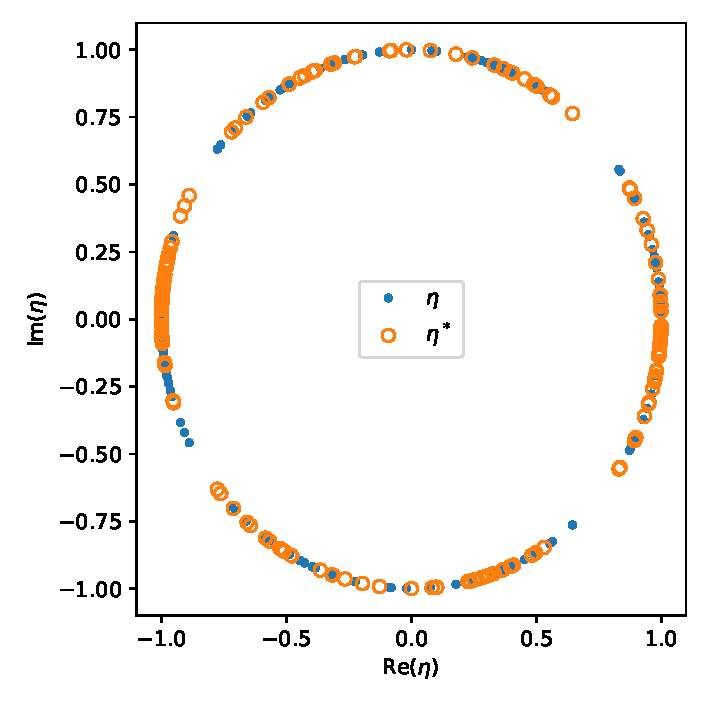
\includegraphics[width=0.44\textwidth]{../Plots/qmbs_sfim_N=08_tduration=6_Vrr=100_Omega=1.pdf}
  }
  \subfigure[PXP]{
    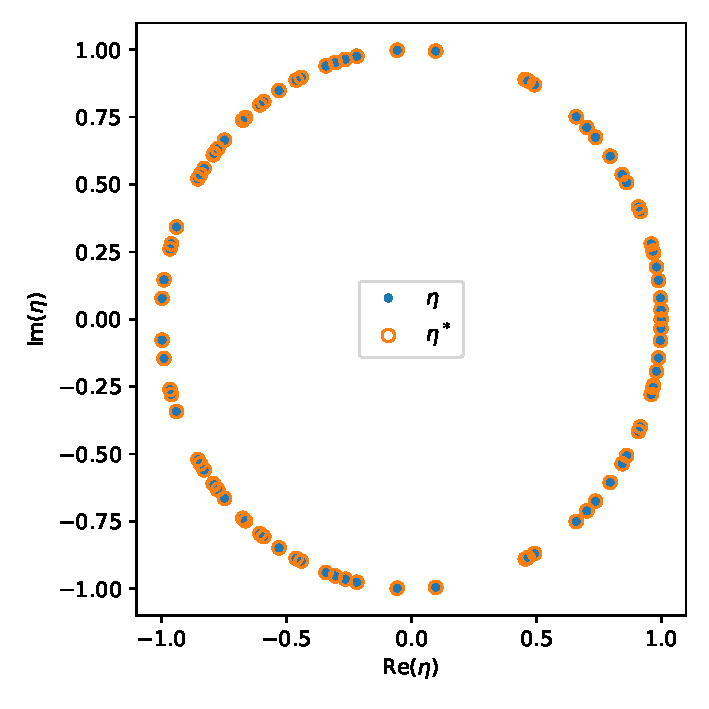
\includegraphics[width=0.44\textwidth]{../Plots/qmbs_pxp_N=08_tduration=6_Omega=1.pdf}
  }
  \caption{Eigenvalues $\eta$ (filled) and their complex conjugates
    $\eta^*$ (open) of the propagator, plotted in the complex plane for
    $N=8$, $\Omega t=6$. (a)~SFI with $V_{rr}=100\Omega$: the
    conjugates are reflections about the real axis, shown as a guide to
    the eye. (b)~PXP: the particle-hole symmetry
    $\Gamma = \prod_{l} Z_{l}$ of the PXP model at $\Delta = 0$ makes
    $\eta^*$ the eigenvalue of the partner state at energy $-E$.}
\end{figure}


\begin{figure}
  \centering
  \subfigure[SFI]{
    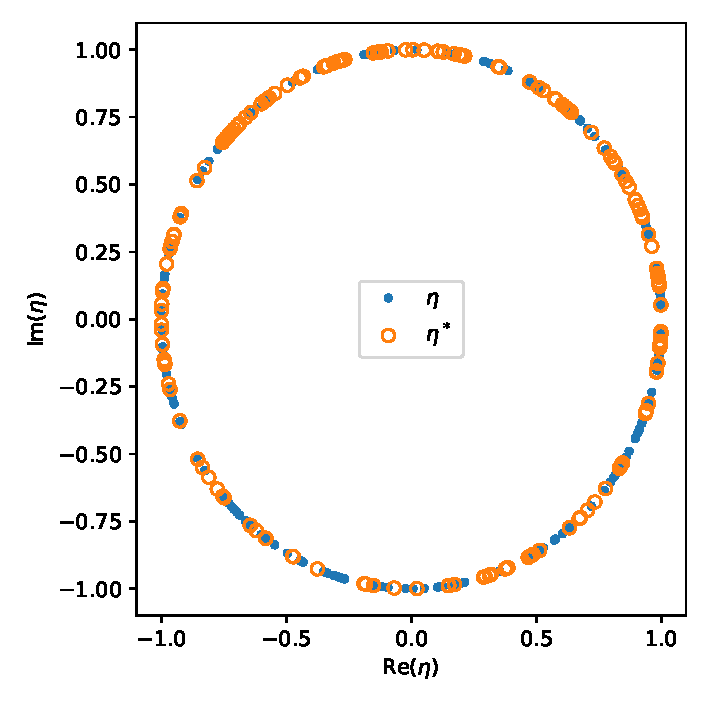
\includegraphics[width=0.44\textwidth]{../Plots/qmbs_sfim_N=08_tduration=11_Vrr=100_Omega=1.pdf}
  }
  \subfigure[PXP]{
    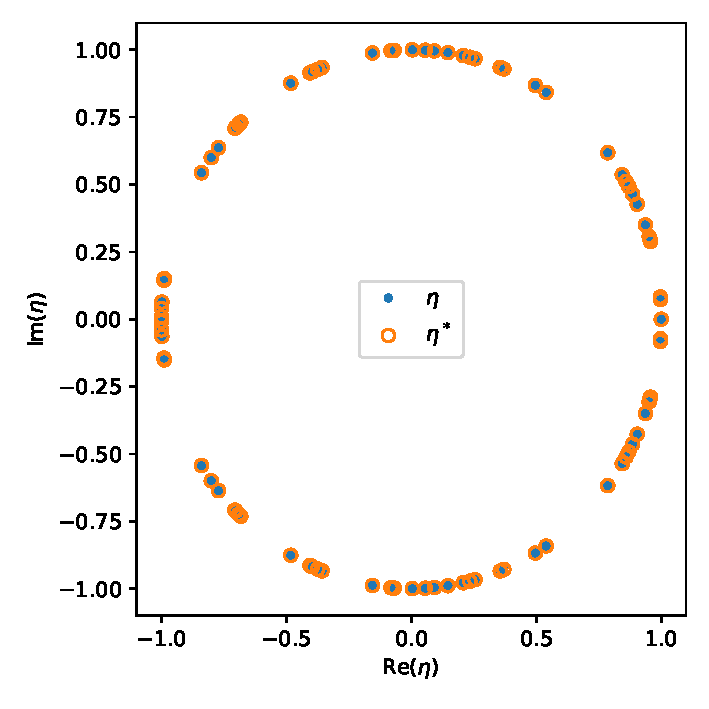
\includegraphics[width=0.44\textwidth]{../Plots/qmbs_pxp_N=08_tduration=11_Omega=1.pdf}
  }
  \caption{Eigenvalues $\eta$ (filled) and their complex conjugates
    $\eta^*$ (open) of the propagator, plotted in the complex plane for
    $N=8$, $\Omega t=11$. (a)~SFI with $V_{rr}=100\Omega$: the
    conjugates are reflections about the real axis, shown as a guide to
    the eye. (b)~PXP: the particle-hole symmetry
    $\Gamma = \prod_{l} Z_{l}$ of the PXP model at $\Delta = 0$ makes
    $\eta^*$ the eigenvalue of the partner state at energy $-E$.}
\end{figure}

%%%%%%%%%%%%%%%

\begin{figure}
  \centering
  \subfigure[SFI]{
    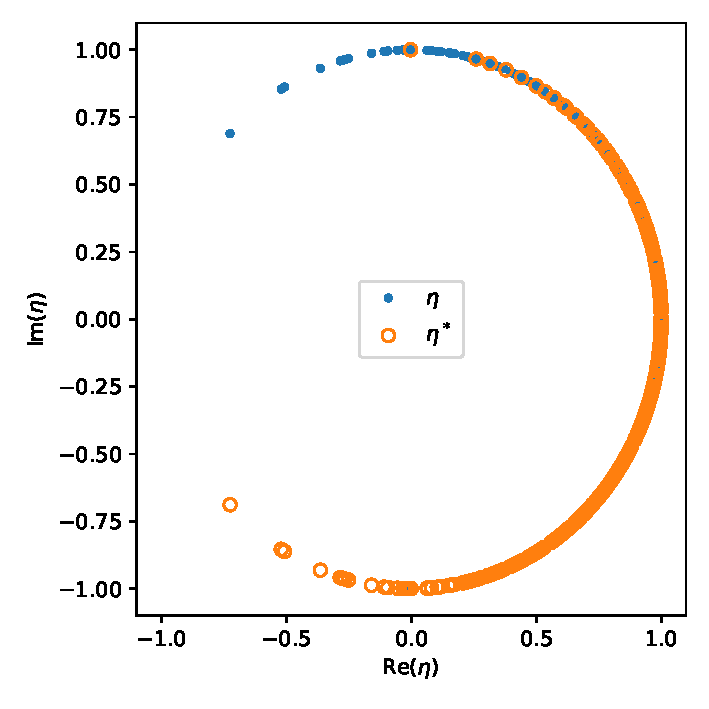
\includegraphics[width=0.44\textwidth]{../Plots/qmbs_sfim_N=10_tduration=0.5_Vrr=100_Omega=1.pdf}
  }
  \subfigure[PXP]{
    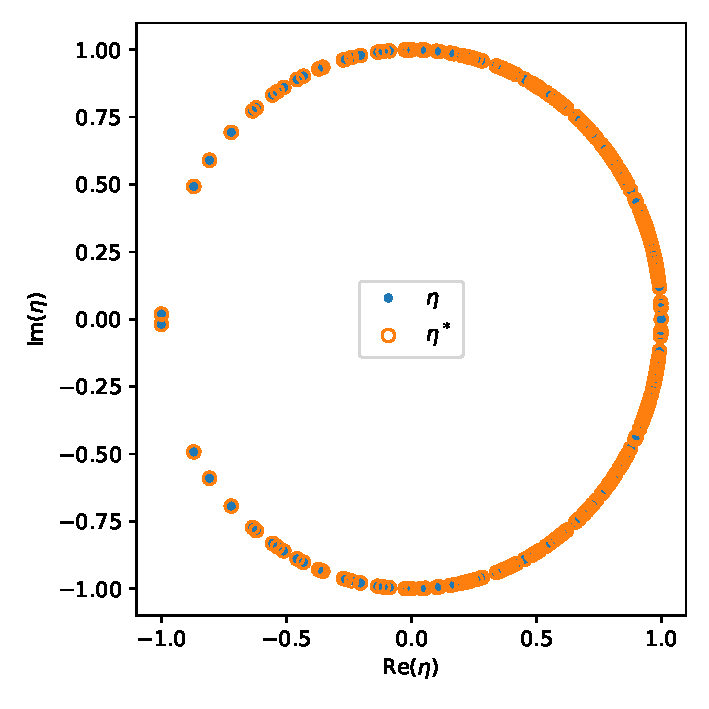
\includegraphics[width=0.44\textwidth]{../Plots/qmbs_pxp_N=10_tduration=0.5_Omega=1.pdf}
  }
  \caption{Eigenvalues $\eta$ (filled) and their complex conjugates
    $\eta^*$ (open) of the propagator, plotted in the complex plane for
    $N=10$, $\Omega t=0.5$. (a)~SFI with $V_{rr}=100\Omega$: the
    conjugates are reflections about the real axis, shown as a guide to
    the eye. (b)~PXP: the particle-hole symmetry
    $\Gamma = \prod_{l} Z_{l}$ of the PXP model at $\Delta = 0$ makes
    $\eta^*$ the eigenvalue of the partner state at energy $-E$.}
\end{figure}

\begin{figure}
  \centering
  \subfigure[SFI]{
    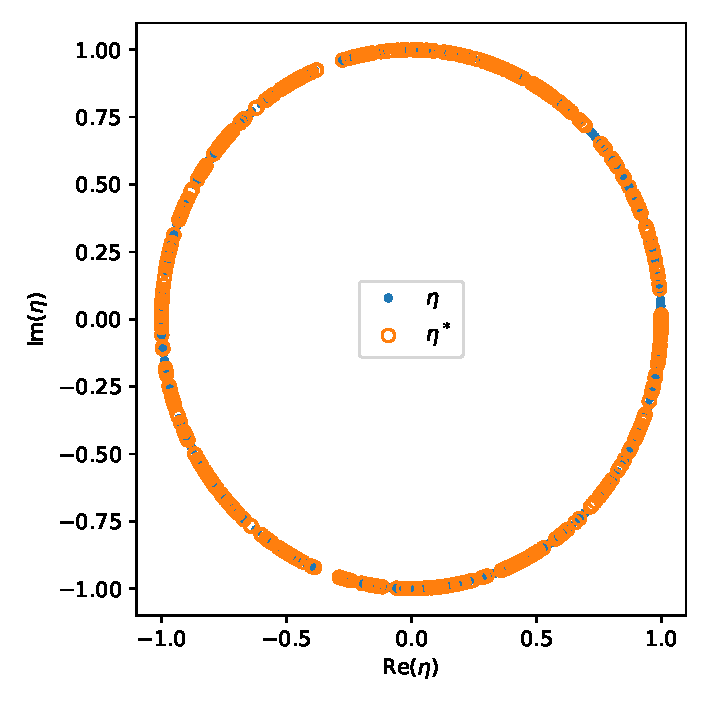
\includegraphics[width=0.44\textwidth]{../Plots/qmbs_sfim_N=10_tduration=2_Vrr=100_Omega=1.pdf}
  }
  \subfigure[PXP]{
    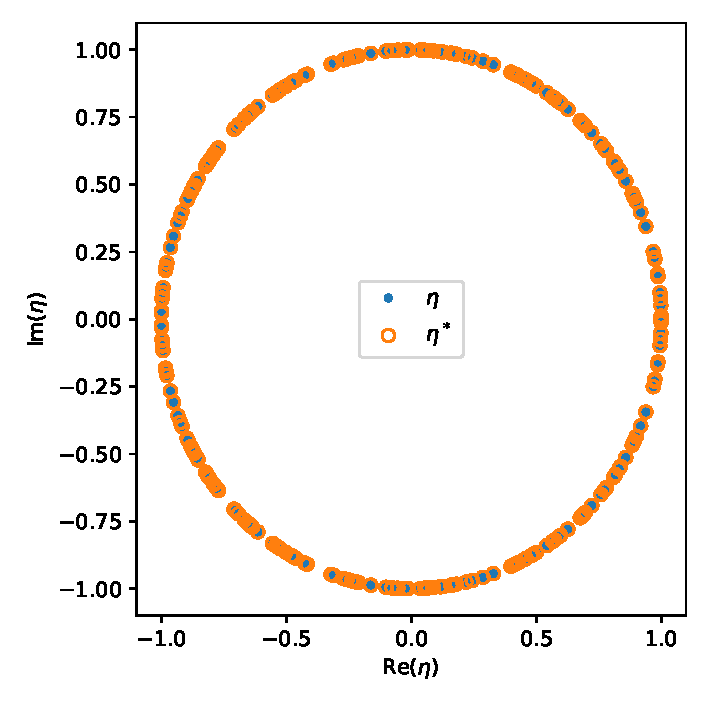
\includegraphics[width=0.44\textwidth]{../Plots/qmbs_pxp_N=10_tduration=2_Omega=1.pdf}
  }
  \caption{Eigenvalues $\eta$ (filled) and their complex conjugates
    $\eta^*$ (open) of the propagator, plotted in the complex plane for
    $N=10$, $\Omega t=2$. (a)~SFI with $V_{rr}=100\Omega$: the
    conjugates are reflections about the real axis, shown as a guide to
    the eye. (b)~PXP: the particle-hole symmetry
    $\Gamma = \prod_{l} Z_{l}$ of the PXP model at $\Delta = 0$ makes
    $\eta^*$ the eigenvalue of the partner state at energy $-E$.}
\end{figure}


\begin{figure}
  \centering
  \subfigure[SFI]{
    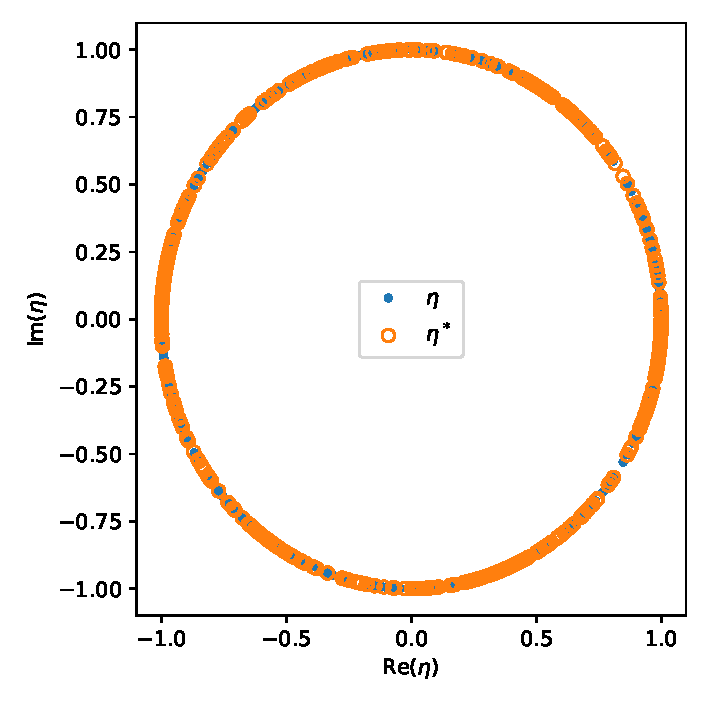
\includegraphics[width=0.44\textwidth]{../Plots/qmbs_sfim_N=10_tduration=6_Vrr=100_Omega=1.pdf}
  }
  \subfigure[PXP]{
    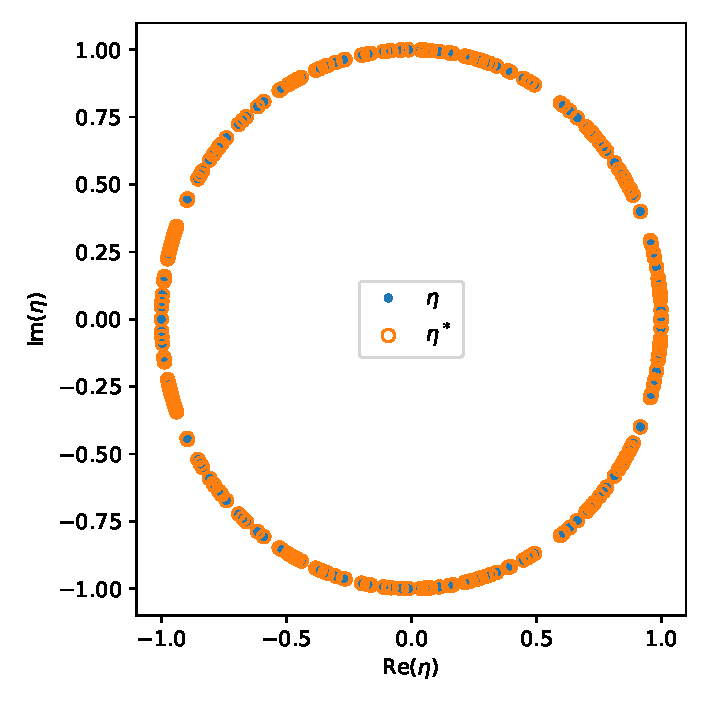
\includegraphics[width=0.44\textwidth]{../Plots/qmbs_pxp_N=10_tduration=6_Omega=1.pdf}
  }
  \caption{Eigenvalues $\eta$ (filled) and their complex conjugates
    $\eta^*$ (open) of the propagator, plotted in the complex plane for
    $N=10$, $\Omega t=6$. (a)~SFI with $V_{rr}=100\Omega$: the
    conjugates are reflections about the real axis, shown as a guide to
    the eye. (b)~PXP: the particle-hole symmetry
    $\Gamma = \prod_{l} Z_{l}$ of the PXP model at $\Delta = 0$ makes
    $\eta^*$ the eigenvalue of the partner state at energy $-E$.}
\end{figure}


\begin{figure}
  \centering
  \subfigure[SFI]{
    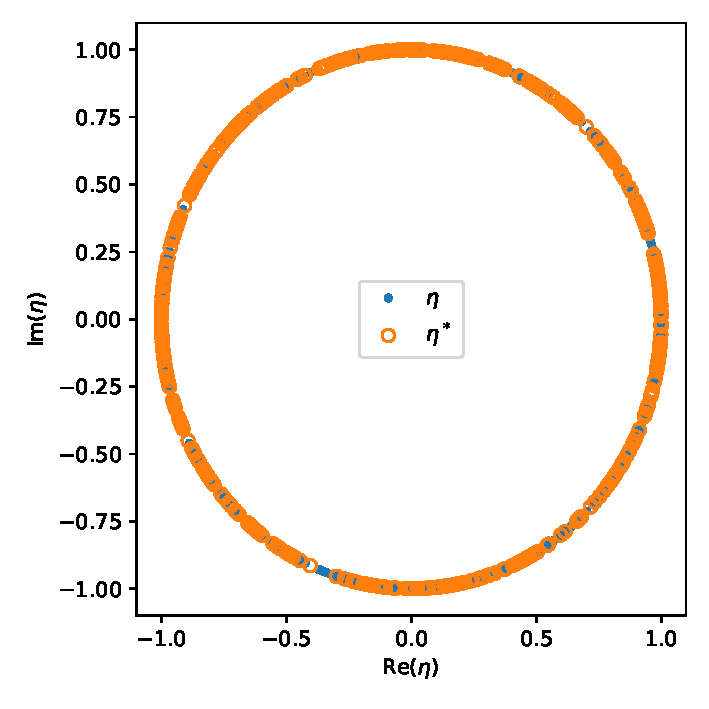
\includegraphics[width=0.44\textwidth]{../Plots/qmbs_sfim_N=10_tduration=11_Vrr=100_Omega=1.pdf}
  }
  \subfigure[PXP]{
    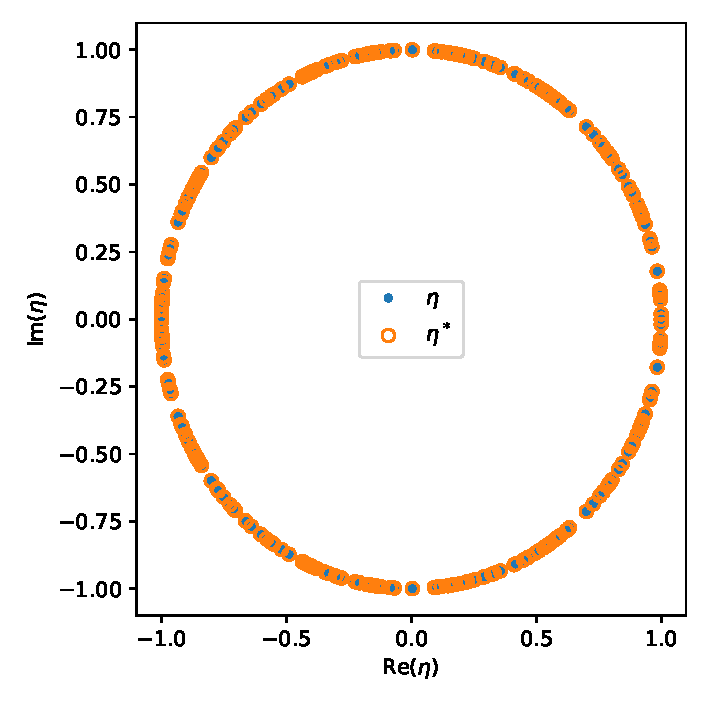
\includegraphics[width=0.44\textwidth]{../Plots/qmbs_pxp_N=10_tduration=11_Omega=1.pdf}
  }
  \caption{Eigenvalues $\eta$ (filled) and their complex conjugates
    $\eta^*$ (open) of the propagator, plotted in the complex plane for
    $N=10$, $\Omega t=11$. (a)~SFI with $V_{rr}=100\Omega$: the
    conjugates are reflections about the real axis, shown as a guide to
    the eye. (b)~PXP: the particle-hole symmetry
    $\Gamma = \prod_{l} Z_{l}$ of the PXP model at $\Delta = 0$ makes
    $\eta^*$ the eigenvalue of the partner state at energy $-E$.}
\end{figure}


\section{Numerical methods}\label{sec:numerical-methods}

All numerical results in this work are produced with the
\texttt{mbl\_eigen} package accompanying this manuscript. The package
combines root-level command-line entry points with a reusable Python
library. QuTiP provides the operator algebra, tensor products, operator
expansion, and partial traces; NumPy and SciPy provide dense linear
algebra and disorder sampling; PyTorch and JAX provide optional
accelerator backends for Hermitian eigendecompositions; and an optional
layer built on Qiskit constructs and simulates the same propagators as
gate-native quantum circuits. The root-level \texttt{main\_*.py} scripts
are compatibility shims: each builds its argument parser from the shared
builders of \texttt{mbl\_eigen.cli} and forwards the parsed arguments to
a package-level runner.

\subsection{Eigenvalue-analysis workflows}\label{subsec:workflows}

\subsubsection{QMBS and PXP eigenphase analysis}

The QMBS workflow (\texttt{mbl\_eigen.qmbs\_app.run\_qmbs}) constructs
two Hamiltonians for a chain of $N$ spin-$1/2$ sites through the builders
of \texttt{mbl\_eigen.qmbs\_model}: a slanted-field-Ising (SFI)
Hamiltonian with a transverse drive, a longitudinal detuning term, and
nearest-neighbor Rydberg-projector interactions, and a constrained PXP
Hamiltonian in which each transverse drive term is flanked by
ground-state projectors on the neighboring sites, with open boundary
conditions. In the conventions of the implementation,
\begin{equation}\label{eq:hsfi-code}
    H_{\mathrm{SFI}}
    = \frac{\Omega}{2}\sum_{l} X_{l}
    + \frac{\Delta}{2}\sum_{l} Z_{l}
    + V_{rr}\sum_{l} P_{r}^{(l)} P_{r}^{(l+1)},
    \qquad
    P_{r} = \frac{\mathbb{I} - Z}{2},
\end{equation}
and
\begin{equation}\label{eq:hpxp-code}
    H_{\mathrm{PXP}}
    = \frac{\Omega}{2}\sum_{l} P_{g}^{(l-1)} X_{l} P_{g}^{(l+1)}
    + \frac{\Delta}{2}\sum_{l} Z_{l},
    \qquad
    P_{g} = \frac{\mathbb{I} + Z}{2}.
\end{equation}
Both Hamiltonians are diagonalized with the selected Hermitian backend
of the eigensolver layer described in Sec.~\ref{subsec:eigensolver}. The
energy eigenvalues $E_n$ are converted into unitary eigenvalues
$\eta_n = \exp(-\im E_n t)$ for the requested duration $t$; the
eigenphases $\arg \eta_n$ are mapped to $[0, 2\pi)$ and sorted; and the
mean adjacent level-spacing ratio defined in
Sec.~\ref{subsec:level-spacing} is computed both for the energy spectra
and for the eigenphase spectra. Finally, the workflow plots the
eigenvalues $\eta_n$ together with their complex conjugates $\eta_n^*$
on the unit circle and writes one figure per Hamiltonian. The shipped
parameter values are $\Omega = 1$ and $V_{rr} = 100\,\Omega$.

\subsubsection{MBL-DTC Floquet analysis}

The MBL-DTC workflow (\texttt{mbl\_eigen.mbldtc\_app.run\_mbldtc})
samples the on-site rotation angles $\varphi_{z,\ell}$ and the
nearest-neighbor interaction angles $\varphi_{zz,\ell}$ independently
and uniformly from $[0, \pi)$, and assembles the Floquet operator of one
drive period as an ordered product of single-site rotation exponentials
and nearest-neighbor interaction exponentials,
\begin{equation}\label{eq:udrive-code}
    U_{\mathrm{drive}}
    = \left[\prod_{\ell=0}^{N-2}
      \exp\left(-\im\, \frac{\varphi_{zz,\ell}}{2}\,
      Z_{\ell} Z_{\ell+1}\right)\right]
    \left[\prod_{\ell=0}^{N-1}
      \exp\left(-\im\, \frac{\varphi_{z,\ell}}{2}\,
      Z_{\ell}\right)\right]
    \left[\prod_{\ell=0}^{N-1}
      \exp\left(-\im\, \frac{\theta_{x}}{2}\,
      X_{\ell}\right)\right],
\end{equation}
where each single-site factor is promoted to the full Hilbert space with
\texttt{qutip.qip.operations.expand\_operator}. Because the Floquet
operator is unitary rather than Hermitian, it is diagonalized with the
general eigenproblem solver of Sec.~\ref{subsec:eigensolver}, which
currently supports the QuTiP backend only. The eigenphases are extracted
and sorted as in the QMBS workflow, the level-spacing ratio is computed
from the Floquet eigenphases, the eigenphases of the squared Floquet
operator $U_{\mathrm{drive}}^{\,2}$ are written to the logging output,
and the eigenvalues $\eta$ are plotted together with their complex
conjugates $\eta^*$, that is, their reflections across the real axis,
on the unit circle. The phase-$\pi$ partners $-\eta$ associated with
period doubling are a related structure and are not plotted separately;
the two descriptions coincide at the DTC point of the dipolar
experiment of Ref.~\cite{choi2017observation}, where the two-to-one
Floquet quasienergies pair as $\pm \varepsilon_i$ and cluster near
$\varepsilon_i \approx \pi/2$, so that the complex conjugate $\eta^*$
and the phase-$\pi$ partner $-\eta$ of an eigenvalue are numerically
equal.

\subsubsection{Random-field MBL workflows}

Three workflows study a random-field MBL model built by
\texttt{mbl\_eigen.mbl\_model}. One disorder realization consists of
nearest-neighbor couplings $J_i$ drawn from a normal distribution with
mean $J$ and standard deviation $\sigma_J$ for $i = 0, \dots, N-2$,
local field magnitudes $B_i$ drawn from a normal distribution with mean
$B$ and standard deviation $\sigma_B$, and field polar angles $\theta_i$
drawn uniformly from $[\theta_{\min}\pi, \theta_{\max}\pi)$. The
Hamiltonian reads
\begin{equation}\label{eq:hmbl}
    H_{\mathrm{MBL}}
    = \sum_{i} B_{i}\sin\theta_{i}\, X_{i}
    + \sum_{i} B_{i}\cos\theta_{i}\, Z_{i}
    + \sum_{i=0}^{N-2} J_{i}\, Z_{i} Z_{i+1}.
\end{equation}

The spectrum workflow (\texttt{mbl\_eigen.mbl\_app.run\_mbl})
diagonalizes $H_{\mathrm{MBL}}$, computes the half-chain von Neumann
entanglement entropy of every eigenstate by partial trace over the first
$\lfloor N/2 \rfloor$ sites (\texttt{qutip.ptrace} and
\texttt{qutip.entropy\_vn}), computes the level-spacing ratios of the
energy spectrum and of the derived eigenphases, and plots the
entanglement entropy against energy together with the maximally mixed
value $\lfloor N/2 \rfloor \ln 2$ as a reference line.

The dynamics workflow (\texttt{mbl\_eigen.mbl\_app.run\_mbl\_dynamics})
expands the initial product state $|1 \ldots 1\rangle$ in the Hamiltonian
eigenbasis, evaluates the return amplitude
\begin{equation}\label{eq:return-amplitude}
    A(t) = \sum_{n} \left| \langle E_n | \psi_0 \rangle \right|^{2}
    e^{-\im E_n t}
\end{equation}
on a uniform time grid with nominal spacing $0.0625$ up to the requested
duration, and plots the return rate
$\lambda(t) = -\ln|A(t)|^{2}/N$.

The propagator workflow
(\texttt{mbl\_eigen.mbl\_app.run\_mbl\_propagator}) converts the
Hamiltonian to a dense array, expands the local operators $X_i$, $Y_i$,
and $Z_i$ to every site normalized by $1/\sqrt{2^{N}}$, rotates them
into the eigenbasis through $V^{\dagger} O V$, where $V$ is the
eigenvector matrix, evolves each rotated operator as
$\tilde{O}(t) = V \exp(-\im D t)\, \tilde{O}\, \exp(\im D t)
V^{\dagger}$, with $D$ the diagonal matrix of phases $\exp(-\im E_n t)$,
so that $O(t) = U(t)\, O\, U(t)^{\dagger}$ with
$U(t) = V \exp(-\im D t) V^{\dagger}$, and computes the overlap matrix
$\operatorname{tr}\!\left[\, O_{\alpha}^{(i)}\, O_{\beta}^{(j)}(t)
\,\right]$ between the initial and time-evolved local operators over all
$x$, $y$, and $z$ channels, sites, and time points on the same grid. The
final-time overlap matrix is written to the logging output; no figure is
saved.

A remark on conventions is in order. The normalization conventions of
the builders described in this section differ from the model definitions
of Secs.~\ref{many-body-localized-discrete-time-crystal}
and~\ref{quantum-many-body-scars}: the interaction exponential in
Eq.~\eqref{eq:udrive-code} carries twice the rotation angle of the
corresponding factor in Eq.~\eqref{eq:mbldtc-notes}; the detuning term
in Eq.~\eqref{eq:hsfi-code} enters with the opposite sign, and the
Rydberg projector is $(\mathbb{I} - Z)/2$ rather than
$(\mathbb{I} + Z_l)/2$ as in Eq.~\eqref{eq:sfi-notes}; and the PXP
builder of Eq.~\eqref{eq:hpxp-code} contains a longitudinal detuning
term and a factor of one half that are absent from
Eq.~\eqref{eq:pxp-notes}. The builders described in this section are the
definitive reference for all numerical results presented in this
manuscript.

\subsection{Eigensolver backends}\label{subsec:eigensolver}

The eigensolver layer (\texttt{mbl\_eigen.eigensolver}) exposes two
entry points: \texttt{solve\_hermitian\_eigenproblem}, which supports
the backends \texttt{qobj} (QuTiP), \texttt{numpy}, \texttt{scipy},
\texttt{torch}, and \texttt{jax}; and
\texttt{solve\_general\_eigenproblem} for non-Hermitian operators,
which currently supports the QuTiP backend only. Before diagonalization
the operator is converted to a complex128 dense array and tested for
Hermiticity; if the test fails, the operator is symmetrized as
$(H + H^{\dagger})/2$ and a warning is logged. Hermitian results are
converted with \texttt{numpy.real\_if\_close}, eigenvalues with
non-negligible imaginary parts are rejected rather than silently
discarded, and the eigenvalues are returned in ascending order with the
eigenvector columns reordered consistently. Requests without
eigenvectors use each backend's eigenvalue-only routine. The returned
\texttt{EigenResult} carries the backend and device labels and provides
helpers to rebuild QuTiP kets and basis-change operators from the raw
eigenvector matrix.

Devices are selected with the choices \texttt{auto}, \texttt{cpu},
\texttt{gpu}, \texttt{cuda}, and \texttt{mps}. The QuTiP, NumPy, and
SciPy backends run on the CPU only; the PyTorch backend resolves CUDA
devices and rejects the Metal performance-shaders path for
eigendecomposition; and the JAX backend enables float64 arithmetic and
maps explicit \texttt{cuda} and \texttt{mps} requests to a matching
accelerator platform. PyTorch and JAX are optional installation extras
and are imported lazily, only when their backends are selected.

\subsection{Level-spacing statistics}\label{subsec:level-spacing}

The module \texttt{mbl\_eigen.level\_repulsion} computes the mean
adjacent level-spacing ratio. Given a sorted spectrum
$\{\lambda_n\}$, the routine removes a fraction
\texttt{fraction\_cutoff} of the levels from each edge of the spectrum
($0.02$ by default; the eigenvalue-analysis workflows use zero, that
is, the full spectrum), forms the adjacent spacings
$s_n = \lambda_{n+1} - \lambda_n$ over the remaining bulk, and returns
\begin{equation}\label{eq:spacing-ratio}
    r = \Big\langle
    \frac{\min(s_n, s_{n+1})}{\max(s_n, s_{n+1})}
    \Big\rangle_{n},
\end{equation}
where the average runs over the bulk spacings. For eigenphase spectra
the optional \texttt{circular\_period} argument, set to $2\pi$ by the
workflows, appends the wraparound spacing
$\lambda_{0} + 2\pi - \lambda_{\max}$ so that the statistic is well
defined for phases on the circle. Spectra with fewer than three bulk
levels, or with a zero adjacent spacing, raise an error; a lenient
wrapper used by the QMBS and MBL-DTC workflows maps these degenerate
cases to a not-a-number result with a logged warning, so that a run can
continue past a degenerate model.

\subsection{Qiskit circuit layer}\label{subsec:qiskit}

An optional layer built on Qiskit (\texttt{mbl\_eigen.qiskit\_propagators}
and \texttt{mbl\_eigen.qiskit\_simulation}) targets gate-based quantum
computers directly. The MBL-DTC Floquet operator of
Eq.~\eqref{eq:udrive-code} is already gate-native: the builder
\texttt{build\_mbldtc\_floquet\_circuit} implements it exactly as a
circuit of \texttt{rx}, \texttt{rz}, and \texttt{rzz} gates in the same
order as the state-vector workflow, a global $X$ rotation layer, then
on-site $Z$ rotations, then nearest-neighbor $ZZ$ interactions, repeated
for a configurable number of drive cycles, and requires no
Trotterization. Time evolution under the random-field MBL Hamiltonian of
Eq.~\eqref{eq:hmbl} is synthesized as a nearest-neighbor Trotter circuit
(\texttt{build\_mbl\_trotter\_step\_circuit},
\texttt{build\_mbl\_trotter\_circuit}) in either first-order form, a
diagonal layer followed by a transverse layer, or second-order form, a
half diagonal layer, a transverse layer, and a half diagonal layer, with
\texttt{rz} and \texttt{rzz} gates implementing the diagonal $Z$/$ZZ$
sector and \texttt{rx} gates the transverse sector. Model site $\ell$ is
mapped to Qiskit qubit $N - 1 - \ell$, so that the circuit matrices
follow the same site ordering as the QuTiP tensor operators.

The simulation engine supports three backends: an exact statevector
backend that requires only the base Qiskit package; an
\texttt{AerSimulator} backend that runs either in exact statevector mode
or shot-based, requiring the optional \texttt{qiskit-aer} extra; and a
fake-backend mode that attaches the noise model of an IBM fake provider,
by default \texttt{FakeManilaV2}, and is always shot-based. For each
requested time point the number of Trotter steps scales as
$\max(1, \mathrm{round}(n_{\mathrm{trotter}} |t|))$. The engine returns
the time grid, the return rate, that is, the Loschmidt echo
$|\langle \psi_0 | \psi(t) \rangle|^{2}$ in the all-ones initial state,
and the site-resolved longitudinal magnetization
$\langle Z_i \rangle(t)$; shot-based observables are estimated from the
empirical count distributions.

\subsection{Output conventions and reproducibility}\label{subsec:reproducibility}

Output filenames are generated centrally in
\texttt{mbl\_eigen.output\_names}. Every workflow appends a random UUID
suffix to each filename, so repeated runs intentionally produce
different filenames. The MBL-DTC and MBL workflows
accept a \texttt{--seed} flag that makes the sampled disorder
reproducible. Regression tests for the package live in \texttt{tests/}
and run with the standard \texttt{unittest} discovery mechanism.
Figures produced by earlier versions of the package use legacy
filenames without an explicit detuning term; the QMBS figures in this
manuscript reference such legacy outputs.

\section{Results: entanglement entropy and level-spacing statistics}\label{sec:results}

TODO

\section{Finite-size scaling and thermodynamic limit}\label{sec:finite-size-scaling}

TODO

\bibliography{references}

\end{document}
